El sistema devuelve al usuario datos sobre las acciones que toma cuando estas generan salidas en la consola, se permite realizar una acción, se está realizando una acción o se necesita información que el usuario medio pueda desconocer.

\subsubsection{Logs de consola}
Cuando el sistema realiza un proceso, se imprimen por pantalla \textit{logs} que puedan resultar informativos. Ver Figura \ref{fig:logs-gui}

\begin{figure}[H]
    \begin{center}
    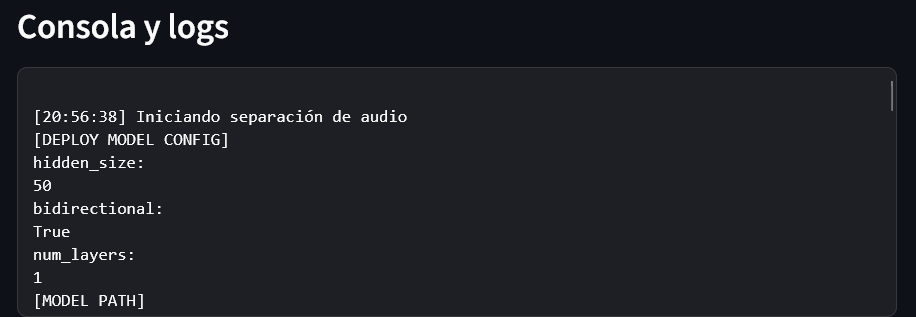
\includegraphics[width=0.7\textwidth]{commons/logs_GUI.png}
    \caption{Ejemplo de \textit{logs} mostrados en la consola de la interfaz}
    \label{fig:logs-gui}
    \end{center}
\end{figure}

\subsubsection{Mensajes de error}
El usuario puede realizar alguna acción que requiera algún paso previo. Si bien no se ha realizado una cobertura exhaustiva de todas las condiciones de error, el sistema muestra mensajes de error en la sección de la interfaz de la Figura \ref{fig:error-gui} en caso de que se produzca alguno de los errores contemplados. 

\begin{figure}[H]
    \begin{center}
    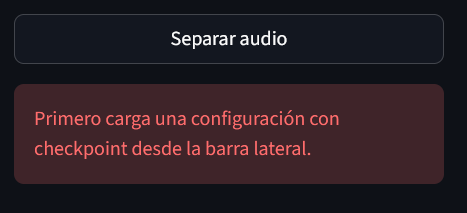
\includegraphics[width=0.7\textwidth]{commons/error_GUI.png}
    \caption{Ejemplo de mensaje de error mostrado en la interfaz al intentar separar una pista sin haber cargado una configuración de modelo previa.}
    \label{fig:error-gui}
    \end{center}
\end{figure}

Los errores que se han contemplado son los siguientes:
\begin{itemize}
    \item No se encuentra ningún checkpoint para la configuración seleccionada.
    \item El checkpoint cargado ya no existe en el disco.
    \item Se intenta separar un audio sin haber cargado un checkpoint.
    \item Se intenta evaluar un modelo sin haber cargado un checkpoint.
    \item No existe alguno de los archivos de audio separados que se han generado.
    \item Falla la generación de la representación gráfica de la onda o del espectrograma de una fuente.
    \item Incompatibilidad entre los pesos del checkpoint y la arquitectura del modelo.
    \item Claves faltantes, inesperadas o con dimensiones incompatibles al cargar un checkpoint.
    \item Fallo al escribir en disco.
    \item Formato o tipo de salida de audio en la separación no soportado.
\end{itemize}

\subsubsection{Progreso}
Mientras se está realizando una acción que requiere de tiempo, como separar una pista, la interfaz muestra un indicador de espera. Ver Figura \ref{fig:carga-gui}.

\begin{figure}[H]
    \begin{center}
    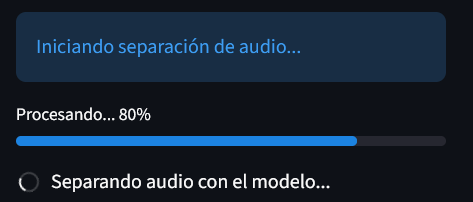
\includegraphics[width=0.7\textwidth]{commons/carga_GUI.png}
    \caption{Ejemplo de indicador de espera en la interfaz mientras se está realizando el proceso de separar una pista.}
    \label{fig:carga-gui}
    \end{center}
\end{figure}

\subsubsection{Descarga de fuentes}
Por cada fuente separada el sistema permite al usuario guardar una copia en su equipo. Esto estaría pensado para una situación real en la que este sistema está alojado en un servidor y no en ejecución local ya que en ejecución local no hace falta descargar nada. Ver Figura \ref{fig:descarga-gui}.

\begin{figure}[H]
    \begin{center}
    
\includegraphics[width=0.7\textwidth]{commons/descarga_GUI.png}
    \caption{Botón de la interfaz que descarga un archivo wav de fuente en el almacenamiento del usuario.}
    \label{fig:descarga-gui}
    \end{center}
\end{figure}
